
%----------------------------------------------------------------------------------------
%	PACKAGES AND OTHER DOCUMENT CONFIGURATIONS
%----------------------------------------------------------------------------------------

\documentclass{beamer}

\usetheme{Goettingen}
\usepackage{algorithm}
\usepackage{algpseudocode}
\usepackage{graphicx}
\usepackage{subcaption}
\usepackage{amsmath}
\usepackage{amsthm}
\usepackage{caption}
\usepackage{biblatex}

% Declare theorem style and numbering
\theoremstyle{plain}
\newtheorem{thm}{Theorem}
\newtheorem{lem}{Lemma}
\newtheorem{corr}{Korrolar}
\theoremstyle{definition}
\newtheorem{defn}[thm]{Definition}
\newtheorem{ex}[thm]{Beispiel}

\newcommand{\mat}[1]{\mathbf{#1}}
\DeclareMathOperator*{\argmax}{arg\,max}
\DeclareMathOperator*{\argmin}{arg\,min}
\newcommand{\norm}[1]{\left\lVert #1 \right\rVert}

%\setbeamertemplate{bibliography item}{\insertbiblabel}

%----------------------------------------------------------------------------------------
%	BEGIN DOCUMENT
%----------------------------------------------------------------------------------------


\begin{document}

\title{Sparse Principal Component Analysis}
\subtitle{for Frequency Data}   
\institute{Institute for Numerical Simulation}
\author{Tobias Bork} 
\date{\today}
\titlegraphic{	\vspace{0.5cm}
				
\includegraphics[scale=0.04]{figures/university_of_bonn.png} 				\hspace{1cm}
				
\includegraphics[scale=0.10]{figures/fraunhofer_scai.png}}

\begin{frame}
\titlepage
\end{frame}


%----------------------------------------------------------------------------------------
%	Introduction
%----------------------------------------------------------------------------------------

\section{Introduction} 
\begin{frame}
\frametitle{Dimensionality Reduction} 

\begin{itemize}
\item \textbf{Problems} in high dimensions: 
\setbeamertemplate{itemize items}[circle]
	\begin{itemize}
	\item Time and storage space
	\item Visualizing data set
	\item Curse of dimensionality
	\end{itemize}
\setbeamertemplate{itemize items}[triangle]
\item \textbf{Idea:} Reduce the number of variables while preserving structure in the data
\item \textbf{Approach:} Feature selection methods
\item \textbf{Approach:} Feature extraction methods

\end{itemize}
\end{frame}

%----------------------------------------------------------------------------------------
%	Principal Component Analysis
%----------------------------------------------------------------------------------------

\section{PCA} 
\subsection{Idea}
\begin{frame}
\begin{figure}
\frametitle{Idea of PCA}
\centering
	\begin{subfigure}{0.45\textwidth}
	\centering
	\captionsetup{justification=centering}
	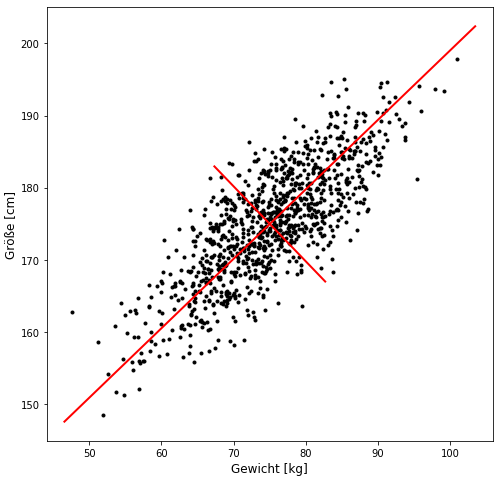
\includegraphics[width = \textwidth]{figures/pca_example.png}
	\caption{Finding principal axis on a data set}
	\end{subfigure}
	%	
	\begin{subfigure}{0.45\textwidth}
	\centering
	\captionsetup{justification=centering}
	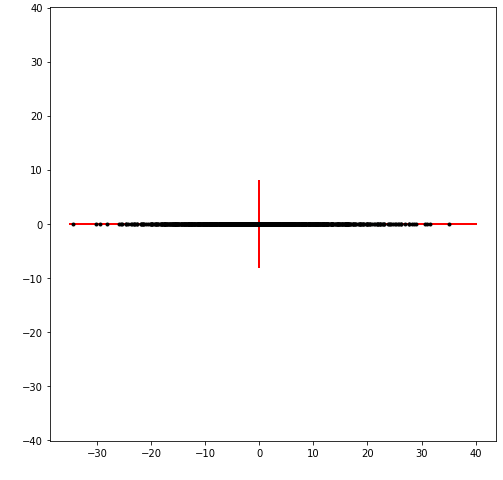
\includegraphics[width = \textwidth]{figures/pca_example_rotated.png}
	\caption{Linear projection of data to first principal axis}
	\end{subfigure}
\end{figure}
\end{frame}

\subsection{Mathematical Formulations}
\begin{frame}
\frametitle{Mathematical Formulation}
Let $\mat X \in \mathbb{R}^{n \times p}$ be a centered data matrix with $n$ samples and $p$ variables. We find the first principal axis by 
$$v_1 = \argmax_{\norm{v}_2 = 1} \text{Var}[\mat{X}v] = \argmax_{\norm{v}_2 = 1} v^T \mat{\Sigma} v$$
where $\mat{\Sigma} = \frac{\mat X^T \mat X}{n}$ is the sample covariance matrix.\pause

We compute the following principal axis successively
$$v_{k+1} = \argmax_{\norm{v} = 1} v^T \mat{\Sigma} v$$ 
$$\text{subject to }v_{k+1}^Tv_l = 0 \quad \forall 1 \leq l \leq k$$\pause
The new principal components are defined by $Z_i = \mat{X}v_i$
\end{frame}

\begin{frame}
\frametitle{Mathematical Formulation using SVD}
The principal axis can also be computed via the eigendecomposition of $\mat{\Sigma}$.
$$\mat{\Sigma} = \mat V \mat L \mat{V}^T$$
where $\mat{L}$ is a diagonal matrix with eigenvalues $\lambda_i$ and $\mat V$ is the matrix of eigenvectors.\linebreak \pause
Closely related is the Singular Value Decomposition (SVD) 
$$ \mat{X} = \mat{U}\mat{D}\mat{V}^T $$
where $\mat{D}$ is a diagonal matrix with singular values $d_1,\ldots,d_p$, $\mat{U}$ a $n \times p$ and $\mat{V}$ a $p \times p$ orthogonal matrix.
\end{frame}

\begin{frame}
\frametitle{PCA as a regression problem}
\begin{figure}
\centering
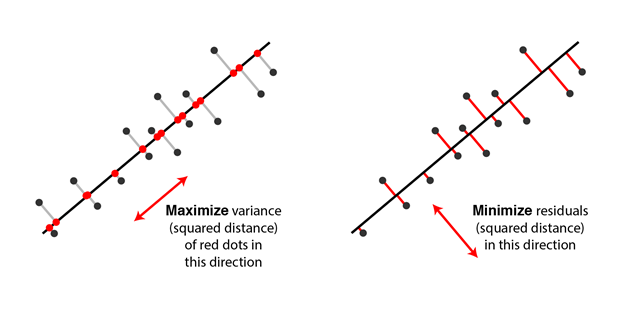
\includegraphics[width = \textwidth]{figures/pca_projection_explanation.png}
\caption{Two equivalent ways of finding principal axis}
\end{figure}
\end{frame}

\begin{frame}
\frametitle{PCA as a regression problem}
\begin{thm} 
Let $x_i$ be the $i$th row of $\mat X$.
$$\mat{\hat{A}}_k = \argmin_{\mat{A}_k} \sum_{i=1}^{n} \norm{x_i - \mat{A}_k \mat{A}_k^Tx_i}^2 + \lambda \sum_{j=1}^{k}\norm{\beta_j}^2$$
$$\text{subject to }\mat{A}_k^T\mat{A}_k = \mat{I}_{k \times k}$$
Then, if we normalize each column $\mat{\tilde{A}}_k = \left[ \frac{\hat{\alpha}_1}{\norm{\hat{\alpha}_1}} \bigg\lvert \cdots \bigg\rvert \frac{\hat{\alpha}_k}{\norm{\hat{\alpha}_1}} \right]$ we recover the first $k$ principal axis.
\end{thm}

\end{frame}
\subsection{Theorems}

\begin{frame}
\frametitle{Theorems}
The Success of PCA is due to the following optimal properties:
\begin{itemize}
\item Principal Components sequentially capture the maximum variability
\item Principal Components are uncorrelated
\item Eckart-Young-Mirsky-Theorem
\end{itemize}
\end{frame}

\subsection{Limits of Usability}
\begin{frame}
\frametitle{Limits of Usability}
\textbf{Drawbacks:}
\begin{itemize}
\item Linear Relationship between variables
\item Completeness of data set
\item Outliers in data set
\item PCA is inconsistent when $p \gg n$
\item Interpreation of principal axis
\end{itemize}


\end{frame}


\subsection{Application}

\begin{frame}
\frametitle{Application to handwritten digits}
\textbf{Data Set Characteristics:}
\begin{itemize}
\item \textbf{Number of Instances:} 1797
\item \textbf{Number of Attributes:} 64
\item \textbf{Attribute Information:} $8 \times 8$ image of integer pixels
\end{itemize}

\begin{figure}
\centering
	\begin{subfigure}{0.45\textwidth}
	\centering
	\captionsetup{justification=centering}
	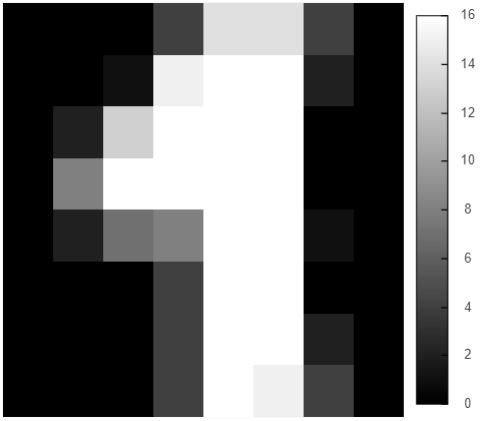
\includegraphics[width = \textwidth]{figures/handwritten_digits_dataset_1.jpg}
	\caption{Handwritten digit 1}
	\end{subfigure}
	%	
	\begin{subfigure}{0.45\textwidth}
	\centering
	\captionsetup{justification=centering}
	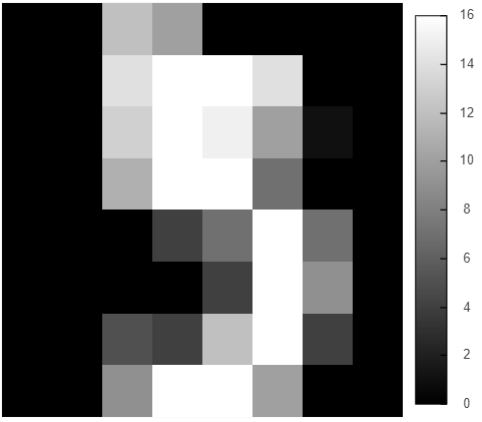
\includegraphics[width = \textwidth]{figures/handwritten_digits_dataset_5.jpg}
	\caption{Handwritten digit 5}
	\end{subfigure}
\end{figure}
\end{frame}

\begin{frame}
\frametitle{Application to handwritten digits}
\begin{figure}
\centering
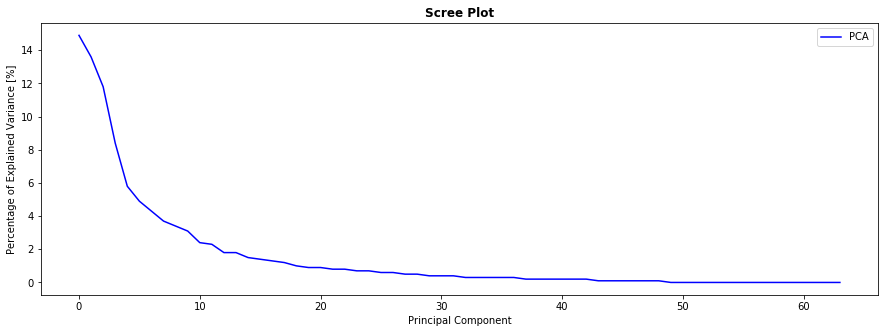
\includegraphics[width = 0.9\textwidth]{figures/pca_handwritten_digits_scree.png}
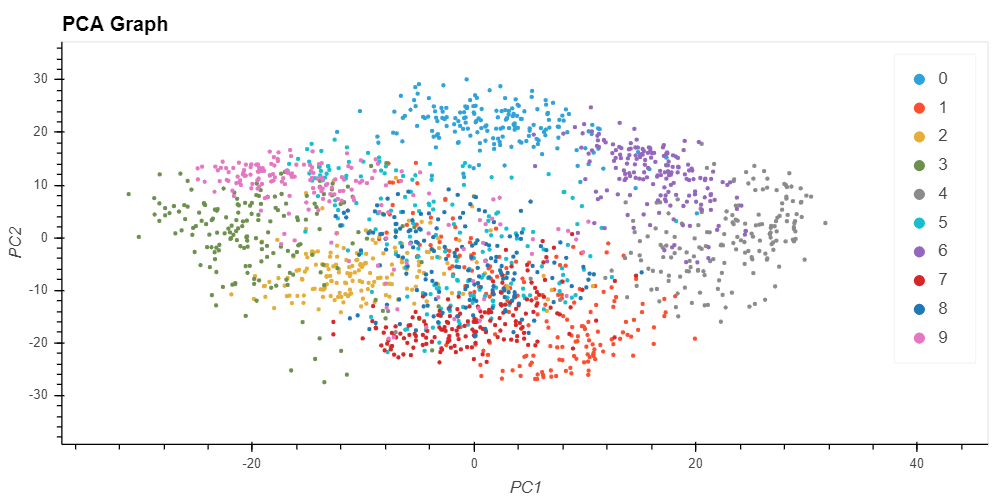
\includegraphics[width = 0.9\textwidth]{figures/pca_handwritten_digits.png}
\end{figure}
\end{frame}


%----------------------------------------------------------------------------------------
%	Sparse Principal Component Analysis
%----------------------------------------------------------------------------------------

\section{Sparse PCA}

\begin{frame}
\frametitle{Sparse PCA}
\textbf{Problem:} Principal Components are hard to interpret \linebreak
\textbf{Approach:} Require sparse loadings when performing PCA

$$\max{v^T \Sigma v}$$
$$\text{subject to } \norm{v}_2 = 1, \quad \norm{v}_{0} \leq t$$

\textbf{Relaxation}:
\begin{itemize}
\item a regression framework
\item a convex semidefinite programming framework
\item a generalized power method framework
\item an alternating maximization framework
\item forward-backward greedy search and exact methods using branch-and-bound techniques
\item Bayesian formulation framework
\end{itemize}
\end{frame}

\subsection{Mathematical Formulation}
\begin{frame}
\frametitle{Mathematical Formulation}
We will use a regression framework to derive sparse PCA.\linebreak

\textbf{Problem Formulation:}\linebreak
Let $\mat B = \left[ \beta_1 \big\vert \cdots \big\vert \beta_k \right]$. The Sparse PCA Criterion is defined by
$$(\hat{\mat{A}}, \hat{\mat{B}}) = \argmin_{\mat{A}, \mat{B}} \sum_{i=1}^{n} \norm{x_i - \mat{A}\mat{B}^Tx_i}^2 + \lambda \sum_{j=1}^{k}\norm{\beta_j}^2 + \sum_{j=1}^k \lambda_{1,j} \norm{\beta_j}_1$$
$$\text{subject to } \mat{A}^T\mat{A} = I_{k \times k}$$

Then, $\beta_i$ represent the newly found sparse principal axis and $Z_i = \mat X \beta_i$ the sparse principal components.
\end{frame}

\subsection{Sparsity and Norms}
\begin{frame}
\frametitle{Sparsity inducing norms}
\begin{figure}
\centering
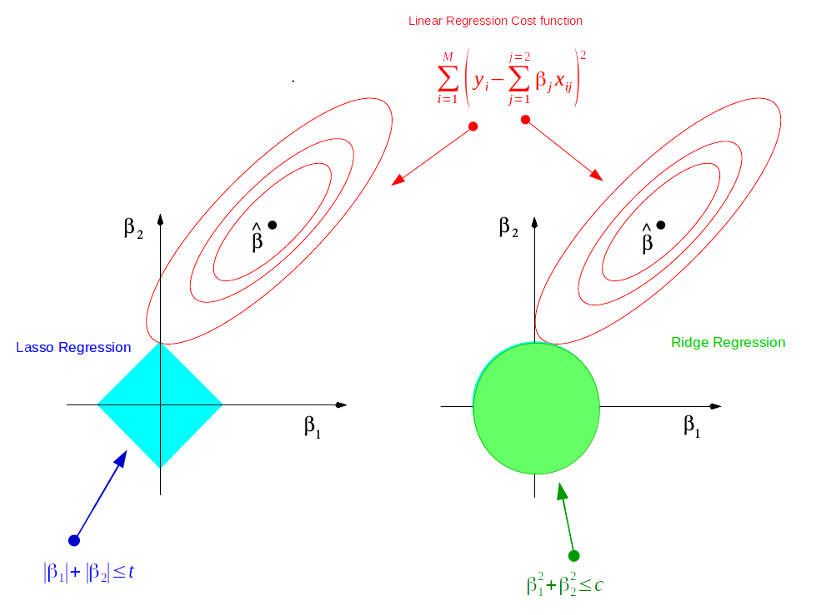
\includegraphics[width = 0.9\textwidth]{figures/lasso_ridge_regression.png}
\end{figure}
\end{frame}

\begin{frame}
\frametitle{Sparsity inducing norms}
\begin{figure}
\centering
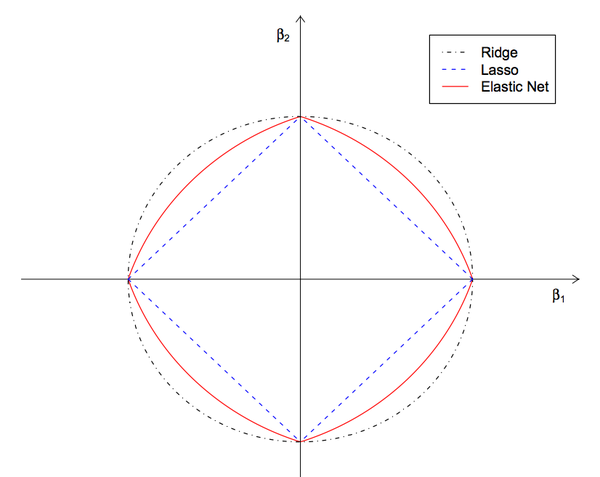
\includegraphics[width = 0.9\textwidth]{figures/lasso_ridge_regression_constraint_region.png}
\end{figure}
\end{frame}

\subsection{Numerical Solution}

\begin{frame}
\frametitle{Numerical Solution}
\textbf{Problem:} How do we minimize the Sparse PCA criterion?\linebreak

$$(\hat{\mat{A}}, \hat{\mat{B}}) = \argmin_{\mat{A}, \mat{B}} \sum_{i=1}^{n} \norm{x_i - \mat{A}\mat{B}^Tx_i}^2 + \lambda \sum_{j=1}^{k}\norm{\beta_j}^2 + \sum_{j=1}^k \lambda_{1,j} \norm{\beta_j}_1$$
$$\text{subject to } \mat{A}^T\mat{A} = I_{k \times k}$$
\end{frame}

\begin{frame}
\begin{itemize}
\item{\textbf{$\mat B$ given $\mat A$:} For each $j$, let $Y^* = \mat X \alpha_j$. We minimize over $\hat{\mat{B}} = \left[ \hat{\beta}_1, \ldots , \hat{\beta}_k\right]$ by solving $k$ elastic net problems
$$\hat{\beta}_j = \argmin_{\beta_j} \norm{Y^* - \mat{X}\beta_j}^2 + \lambda \norm{\beta_j}^2 + \lambda_{1,j} \norm{\beta_j}_1$$} \pause
\item{\textbf{$\mat A$ given $\mat B$:} We can ignore the penalties and minimize
$$\sum_{i=1}^{n} \norm{x_i - \mat{A}\mat{B}^Tx_i}^2 = \norm{\mat{X} - \mat{X} \mat{B} \mat{A}^T}_F^2$$
$$\text{subject to } \mat{A}^T\mat{A} = I_{k \times k}$$
This problem has an explicit solution which is obtained by computing the SVD of
$$(\mat X^T \mat X) \mat B = \mat U \mat D \mat V^T$$
}
\end{itemize}
\end{frame}

\begin{frame}
\begin{thm}[Reduced Rank Procrustes Rotation]
Let $\mat M \in \mathbb{R}^{n \times p}$ and $\mat N \in \mathbb{R}^{n \times k}$ be two matrices. Consider the constrained minimization problem
$$\hat{\mat{A}} = \argmin_{\mat A} \norm{\mat M - \mat N \mat A^T}_F^2 \quad \text{subject to } \mat{A}^T\mat{A} = I_{k \times k}$$
Suppose the SVD of $\mat M^T \mat N$ is $\mat U \mat D \mat V^T$, then 
$$\hat{\mat{A}} = \mat U \mat V^T.$$
\end{thm}
\end{frame}

\begin{frame}
\begin{algorithm}[H]
  \scriptsize
    \caption{General SPCA Algorithm}
    \begin{algorithmic}[1]
        \Procedure{SPCA}{$A,B$}
        	\State $\mat A \gets \mat V[,1 \colon k]$, the loadings of the first k ordinary principal components
            \While{not converged}
                \State Given a fixed $\mat A = [\alpha_1, \ldots, \alpha_k]$, solve $k$ elastic net problems $$\beta_j = \argmin_{\beta} \norm{\mat X \alpha_j - \mat X \beta}^{2} + \lambda \norm{\beta}^2 + \lambda_{1,j}\norm{\beta}_{1}$$
                \State For a fixed $\mat B = [\beta_1, \ldots, \beta_k]$, compute the SVD of $$\mat X^T \mat X \mat B = \mat U \mat D \mat V^T$$
                $$\mat A \gets \mat U \mat V^T$$
            \EndWhile
            \State $\hat{V}_j \gets \frac{\beta_j}{\norm{\beta_j}}$ for $j = 1, \ldots, k$
        \EndProcedure
    \end{algorithmic}
\end{algorithm} 
\end{frame}

\subsection{Application}
\begin{frame}
\end{frame}

\subsection{Further Analysis}
\begin{frame}
\frametitle{Further Analysis}
\begin{itemize}
\item Consistency theorem for Sparse PCA when $p \gg n$
\item Efficient implementation when $p \gg n$
\item Computation of ajusted variances
\item Identify differences in Sparse PCA implementations across different platforms (R, Python)
\item Application to frequency data set
\end{itemize}
\end{frame}


%----------------------------------------------------------------------------------------
%	References
%----------------------------------------------------------------------------------------

\section{References}

\begin{frame}{Bibliography}
\frametitle{References}
\begin{thebibliography}{9}

\bibitem{zou}
  Hastie et al.
  \textit{The Elements of Statistical Learning: Data Mining, Inference, and Prediction}.
  2nd edition. 
  2009,.
  Springer-Verlag New York.
  
 \bibitem{zou_sparsepca}
 Zou et al.
  \textit{Sparse Principal Component Analysis}.
  Journal of Computational and Graphical Statistics.
  Volume 15.
  Number 2.
  2006.
  \textit{https://doi.org/10.1198/106186006X113430}.
  
  \bibitem{foucart}
 Foucart, Rauhut.
 \textit{A Mathematical Introduction to Compressive Sensing}.
 1st edition.
 2013.
 Birkh{\"a}user Basel.

\end{thebibliography}


\end{frame}


%----------------------------------------------------------------------------------------
%	Appendix
%----------------------------------------------------------------------------------------

\section{Appendix}

\begin{frame}
\begin{thm}[Eckart-Young-Mirsky-Theorem]
Let $\widehat{\mat{A}}^* = \mat{U}_1 \mat{D}_1 \mat{V}_1^{\top}$
be the \textit{truncated singular value decomposition}. Then $\widehat{ \mat{A}}^*$ solves the matrix rank approximation problem

$$\min_{\operatorname{rank}(\widehat{\mat{A}}) \leq r} \|\mat{A}-\widehat{\mat{A}}\|_{\text{F}} = \|\mat{A}-\widehat{\mat{A}}^*\|_{\text{F}} = \sqrt{\sigma^2_{r+1} + \cdots + \sigma^2_m}$$

where $\sigma_i$ are the singular values of $\mat A$.
\end{thm}
\end{frame}

\begin{frame}
\frametitle{Linear Regression}
Consider a linear regression model with $n$ observations and $p$ predictors. Let $Y = (y_1, \ldots , y_n)^T$ be the response vector and $\mat X = \left[X_1 \vert \cdots \vert X_p \right]$.\linebreak

The linear regression model has the form
$$f(\mat X) = \beta_0 + \sum_{j=1}^p X_j\beta_j$$
where the $\beta_j$'s are unknown coefficients.

We define the residual sum of squares
$$RSS(\beta) = \sum_{i=1}^n (y_i - f(x_i))^2 = \sum_{i=1}^n (y_i - \beta_0 - \sum_{j=1}^p x_{ij}\beta_j)^2$$
\end{frame}

\begin{frame}
\frametitle{Ridge Regression}
\textbf{Problem Formulation}
$$\hat{\beta}^{ridge} = \argmin_{\beta} \norm{Y - \mat{X}\beta}_{2}^{2} + \lambda \quad \text{subject to } \norm{\beta}_{2}^2 \leq t$$
or equivalently in Lagrangian Form
$$\hat{\beta}^{ridge} = \argmin_{\beta}\left\{\frac{1}{2}\sum_{i=1}^n (y_i - \beta_0 - \sum_{j=1}^p x_{ij}\beta_j)^2 + \lambda\norm{\beta}_{2}^2 \right\}$$
\end{frame}

\begin{frame}
\frametitle{LASSO Regression}
\textbf{Problem Formulation}
$$\hat{\beta}^{lasso} = \argmin_{\beta} \norm{Y - \mat{X}\beta}_{2}^{2} + \lambda \quad \text{subject to } \norm{\beta}_{1} \leq t$$
or equivalently in Lagrangian Form
$$\hat{\beta}^{lasso} = \argmin_{\beta}\left\{\frac{1}{2}\sum_{i=1}^n (y_i - \beta_0 - \sum_{j=1}^p x_{ij}\beta_j)^2 + \lambda\norm{\beta}_{1} \right\}$$
\end{frame}

\begin{frame}
\frametitle{Elastic Net}
The elastic net penalty is a convex combination of the ridge and lasso penalties.\linebreak

\textbf{Problem Formulation:}
$$\hat{\beta}^{en} = \argmin_{\beta} (1 + \lambda_2) \left\{\norm{Y - \mat X \beta}^2 + \lambda_2 \norm{\beta}_{2}^2 + \lambda_1 \norm{\beta}_{1} \right\}$$
Given a fixed $\lambda_2$, the LARS-EN algorithm (Zou and Hastie 2005) efficiently solves the elastic net problem for all $\lambda_1$
with the computational cost of a single least squares fit.
\end{frame}

\begin{frame}
\frametitle{Sparse PCA Algorithm Complexity}
\begin{itemize}
\item \textbf{Case 1: $n > p$}
\begin{itemize}
\item Compute the $p \times p$ matrix $\hat{\mat \Sigma} = \mat X^T \mat X$ which requires $np^2$ operations (Same $\hat{\mat \Sigma}$ is used in each step)
\item Compute $\mat X^T \mat X \mat B$ which costs $p^2k$ operations
\item Compute the SVD of $\mat X^T \mat X \mat B$ which costs $\mathcal{O}(pk^2)$
\item Compute each elastic net solution which requires at most $\mathcal{O}(p^3)$
\end{itemize}
Since $k \leq p$, the total computation cost is at most $np^2 + m\mathcal{O}(p^3)$ where $m$ is the number of iterations before convergence
\end{itemize}
\end{frame}

\begin{frame}
\frametitle{Sparse PCA Algorithm Complexity}
\begin{itemize}
\item \textbf{Case 2: $p \gg n$}\linebreak
The trick of using $\hat{\mat \Sigma}$ is no longer applicable, because $\hat{\mat \Sigma}$ is a huge $p \times p$ matrix in this case. The most consuming step is solving each elastic net, whose cost is of order $\mathcal{O}(pnJ + J^3)$ for a positive $\lambda$, where $J$ is the number of nonzero coeffiecients.

Generally speaking the total cost is of order $mk\mathcal{O}(pnJ+J^3)$, which can be expensive for large $J$ and $p$. Fortunately, there exists a special SPCA algorithm for efficiently dealing with $p \gg n$ data.
\end{itemize}
\end{frame}

\begin{frame}
\frametitle{Numerical Solution}
Let $\mat{A}_{p \times k} = \left[ \alpha_1, \ldots , \alpha_k\right]$ and $\mat{B}_{p \times k} = \left[ \beta_1, \ldots , \beta_k\right]$. Since $\mat A$ is orthonomal, let $\mat A_{\perp}$ be any orthonormal matrix such that $\left[ \mat A ; \mat A_{\perp} \right]$ is $p \times p$ orthonormal. Then we ran reformulate the problem
\begin{align*}
\sum_{i=1}^{n} \norm{x_i - \mat{A}\mat{B}^Tx_i}^2 & = \norm{\mat{X} - \mat{X} \mat{B} \mat{A}^T}_F^2\\
& = \norm{\mat X \mat A_{\perp}}_F^2 + \norm{\mat X \mat A - \mat X \mat B}_F^2\\
& = \norm{\mat X \mat A_{\perp}}_F^2 + \sum_{j=1}^{k} \norm{\mat X \alpha_j - \mat X \beta_j}^2
\end{align*}

\end{frame}



\end{document}
